\documentclass[tikz,border=3.14pt]{standalone}
\usetikzlibrary{3d,decorations.text,shapes.arrows,positioning,fit,backgrounds}
\tikzset{
    pics/fake box/.style args={#1 with dimensions #2 and #3 and #4}{
        code={
            \draw[gray,ultra thin,fill=#1] (0,0,0) coordinate(-front-bottom-left) --++
                (0,#3,0) --++
                (#2,0,0) --++
                (0,-#3,0) -- cycle;
            \draw[gray,ultra thin,fill=#1] (0,#3,0) --++
                (0,0,#4) --++
                (#2,0,0) --++
                (0,0,-#4) -- cycle;
            \draw[gray,ultra thin,fill=#1!80!black] (#2,0,0) --++
                (0,0,#4) --++
                (0,#3,0) --++
                (0,0,-#4) -- cycle;
        }
    },
    circle dotted/.style={dash pattern=on .05mm off 2mm,line cap=round}
}

\begin{document}

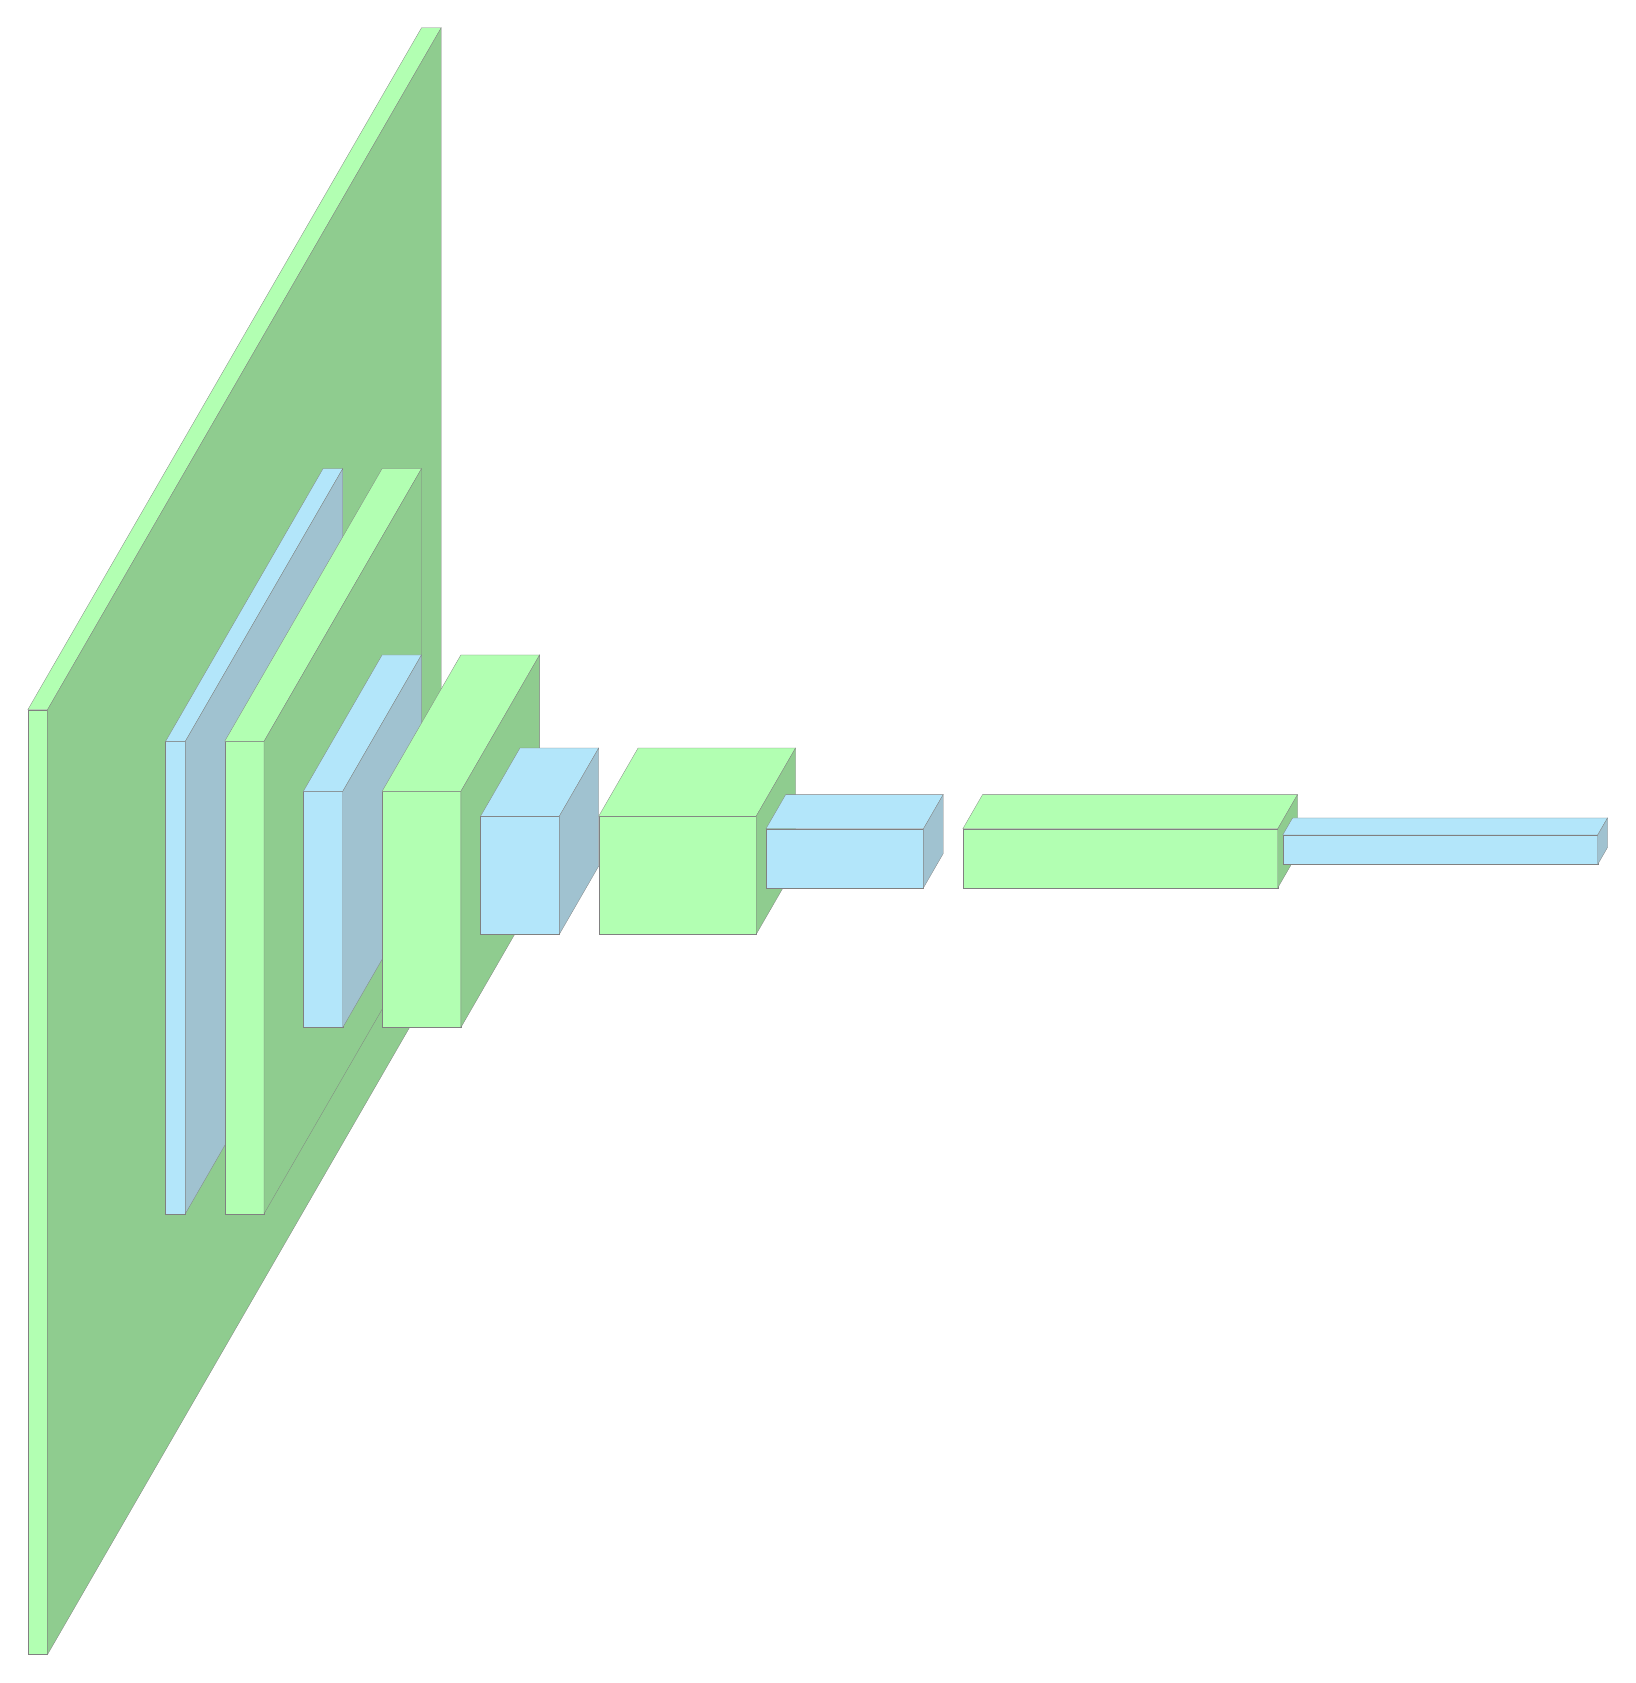
\begin{tikzpicture}[x={(1,0)},y={(0,1)},z={({cos(60)},{sin(60)})},
    font=\sffamily\small,scale=2]

% ========= Convolutional Blocks =========
% image input
% \pic at (-1.5,0,0) {fake box=white!70!gray with dimensions 0 and 12 and 10};

% == CONV1 ==%
\pic at (0, 0,0) {fake box=white!70!green with dimensions 0.25 and 12 and 10};
\pic at (0.125, 1.5, 1.5) {fake box=white!70!cyan with dimensions 0.25 and 6 and 4};
% \draw[-latex,thick] (0.25, 3, 2.5) --++ (0.75, 0, 0);
% \node[above] at (0.4, 2.1, 0) {Block 1};

% == CONV2 ==%
\pic at (0.5, 1.5, 1.5) {fake box=white!70!green with dimensions 0.5 and 6 and 4};
\pic at (0.75, 2.25, 2) {fake box=white!70!cyan with dimensions 0.5 and 3 and 2};
% \draw[-latex,thick] (2, 3, 2.5) --++ (0.5, 0, 0);

% == CONV3 ==%
\pic at (1.25, 2.25, 2) {fake box=white!70!green with dimensions 1.0 and 3 and 2};
\pic at (1.75, 2.625, 2.25) {fake box=white!70!cyan with dimensions 1.0 and 1.5 and 1.0};
% \draw[-latex,thick] (3.75, 3, 2.5) --++ (0.625, 0, 0);

% == CONV4 ==%
\pic at (2.5, 2.625, 2.25) {fake box=white!70!green with dimensions 2.0 and 1.5 and 1.0};
\pic at (3.5, 2.8125, 2.375) {fake box=white!70!cyan with dimensions 2.0 and 0.75 and 0.5};
% \draw[-latex,thick] (6.5, 3, 2.5) --++ (0.75, 0, 0);

% == CONV5 ==%
\pic at (4.75, 2.8125, 2.375) {fake box=white!70!green with dimensions 4.0 and 0.75 and 0.5};
\pic at (6.75, 2.90625, 2.4375) {fake box=white!70!cyan with dimensions 4.0 and 0.375 and 0.25};

% \pic at (1.5,0,0) {fake box=white!70!gray with dimensions 0.8 and 1.6 and 1.2};
% % \node[above] at (1.9, 1.7, 0) {Block 2};

% \draw[-latex,thick] (2.3,0.8,0.5) --++ (0.7,0,0);

% \pic at (3.0,0,0) {fake box=white!70!gray with dimensions 0.8 and 1.2 and 1.0};
% \node[above] at (3.4, 1.3, 0) {Block 3};

% \draw[-latex,thick] (3.8,0.6,0.5) --++ (0.7,0,0);

% \pic at (4.5,0,0) {fake box=white!70!gray with dimensions 0.8 and 1.0 and 0.8};
% \node[above] at (4.9, 1.1, 0) {Block 4};

% \draw[-latex,thick] (5.3,0.5,0.5) --++ (0.7,0,0);

% \pic at (6.0,0,0) {fake box=white!70!gray with dimensions 0.8 and 0.8 and 0.6};
% \node[above] at (6.4, 0.9, 0) {Block 5};

% \draw[-latex,thick] (6.8,0.4,0.5) --++ (0.7,0,0);

% ========= SE Block =========
% \node[draw, single arrow, orange, fill=orange!30, minimum height=0.8cm, minimum width=1cm] (SE) at (8,0,0) {SE};

% \draw[-latex,thick] (7.5,0.5,0.5) -- (SE.west);

% ========= GAP =========
% \node[draw, single arrow, orange, fill=orange!50, minimum height=0.8cm, minimum width=1.2cm] (GAP) at (9.2,0,0) {GAP};

% \draw[-latex,thick] (SE.east) -- (GAP.west);

% ========= Fully Connected Layers =========
% \node[circle,draw,blue,fill=blue!30,minimum size=0.5cm,right=1.2cm of GAP] (FC1) {};
% \node[circle,draw,red,fill=red!30,below=0.6cm of FC1] (FC2) {};
% \node[circle,draw,green,fill=green!30,below=0.6cm of FC2] (FC3) {};
% \draw[circle dotted, line width=2pt,shorten <=3pt] (FC2) -- (FC3);

% \draw[-latex,thick] (GAP.east) -- (FC1.west);

% ========= Dense Output =========
% \node[circle,draw,gray,fill=gray!20,right=1.2cm of FC1] (D1) {};
% \node[circle,draw,gray,fill=gray!60,below=0.6cm of D1] (D2) {};
% \node[circle,draw,gray,fill=gray!20,below=0.6cm of D2] (D3) {};
% \draw[circle dotted, line width=2pt,shorten <=3pt] (D2) -- (D3);

% \foreach \X in {FC1, FC2, FC3}
% {
%     \draw[-latex,thick] (\X) -- (D2.west);
% }

% ========= Background highlighting =========
% \begin{scope}[on background layer]
%     \node[orange!20,rounded corners,fit=(FC1) (FC3),inner sep=8pt]{};
%     \node[gray!10,rounded corners,fit=(D1) (D3),inner sep=8pt]{};
% \end{scope}

\end{tikzpicture}

\end{document}